\documentclass{article}

\usepackage{arxiv}

\usepackage[utf8]{inputenc} % allow utf-8 input
\usepackage[T1]{fontenc}    % use 8-bit T1 fonts
\usepackage{hyperref}       % hyperlinks
\usepackage{url}            % simple URL typesetting
\usepackage{booktabs}       % professional-quality tables
\usepackage{amsfonts}       % blackboard math symbols
\usepackage{nicefrac}       % compact symbols for 1/2, etc.
\usepackage{microtype}      % microtypography
\usepackage{lipsum}
\usepackage{graphicx}	% Including figure files
\usepackage{mathtools}  %loads amsmath as well
\usepackage{amssymb}	% Extra maths symbols
\usepackage[utf8]{inputenc}
\usepackage[english]{babel}
\usepackage{float}
\usepackage{bm}
\usepackage{indentfirst}
\usepackage{tikz}
\usetikzlibrary{positioning}
\usepackage{pgfplots}
\usepackage{color,soul}
\pgfplotsset{compat=1.12}
\definecolor{mygray}{RGB}{225,225,225}
\definecolor{myred}{RGB}{255,60,60}
\definecolor{myblue}{RGB}{60,60,255}

\title{Multiresolution-Enhanced Block-Structured Adaptive Mesh Refinement}


\author{
  Brandon Gusto\\
  Department of Scientific Computing\\
  Florida State University\\
  Tallahassee, FL 32306 \\
  \texttt{bgusto@fsu.edu} \\
  %% examples of more authors
  \And
  Tomasz Plewa \\
  Department of Scientific Computing\\
  Florida State University\\
  Tallahassee, FL 32306 \\
  \texttt{tplewa@fsu.edu} \\
}

\begin{document}
\maketitle

\begin{abstract}
    We present a generalization of Harten's multiresolution scheme for solving
    multiphysics problems on Cartesian, block-structured adaptive mesh
    refinement (AMR) grids. The scheme addresses a shortcoming of tree-based AMR
    codes, which is the creation of blocks with a low filling factor; that is,
    many cells in such a block are resolved beyond the desired error tolerance.
    To overcome this issue, a multiresolution (MR) representation is introduced
    not only to adapt grid but also to select fluxes which may be interpolated
    from the MR basis.  The flux interpolation error introduced by this
    approximation is of the same order as the local truncation error of the
    reconstruction scheme. Thus the rate of convergence of the underlying
    spatial reconstruction scheme is preserved.  This procedure can be easily
    incorporated into existing parallel codes.  Additionally, the MR transform
    is applied per AMR block, obviating any need for communication of MR
    information between blocks. The efficiency of the scheme is demonstrated
    using several one and two-dimensional problems.
\end{abstract}

% keywords can be removed
\keywords{Multiresolution \and Adaptive Mesh Refinement \and Conservation Laws}

\section{Introduction}
    % paragraph introduces the need for spatially adaptive grids
    The dynamics of reactive flows are typically characterized by disparate
    spatial and temporal length scales. Certain features of the flow such as
    shocks, material discontinuities, or burning fronts often require
    significantly higher spatial resolution than other regions of the flow.
    Naturally, intense effort has gone into the development of methods which
    employ a multi-scale or adaptive strategy to accurately simulate such flows without
    over-resolving large areas of the domain.

    % paragraph introducing adaptive mesh refinement as a concept
    Methods which introduce a hierarchy of nested grid levels are generally
    described as adaptive mesh refinement (AMR) methods. Obtaining an estimate
    of the local truncation error (LTE) of the reconstruction scheme on a
    particular grid level enables the scheme to identify regions where
    refinement is necessary. AMR methods may employ several strategies to
    approximate the LTE. The earliest work utilized gradient information to flag
    cells for refinement \cite{Berger1984}.  Alternative methods include
    feature-based refinement, and evaluation of gradient information (references
    here).

    % paragraph reviews the work of harten and multiresolution methods
    In a seminal paper, Harten (cite) introduced a scheme based on
    multiresolution (MR) analysis for numerically solving hyperbolic partial
    differential equations. The MR scheme represents the discrete solution on a
    set of nested grids using the MR basis. This basis is constructed using
    average-interpolating wavelets

    Other methods are based on multiresolution analysis, refining the grid based on
    the absolute value of wavelet coefficients (\hl{long list of papers, harten,
    chiavassa, domingues, bla bla}).

\section{Multiresolution Analysis}
A multiresolution analysis (MRA) provides a hierarchy of nested
approximation spaces to construct a basis in $L^2(\mathbb{R}^\mathbf{d})$.
While a Fourier basis decomposes a signal into only frequency components,
a wavelet basis captures both frequency and spatial localization. A MRA is
defined by a sequence of nested subspaces
\begin{equation*}
\dots \subset V_{j-1} \subset V_{j} \subset V_{j+1} \subset \dots \text{ }
\text{ } \text{ } \text{ } j\in \mathbb{Z},
\end{equation*}
where each subspace $V_{j}$ is associated with a set of points $\gamma_{j}$.
In the finite dimensional setting, a given signal is split
into odd and even components, and regularity information is obtained
by the accuracy of the prediction of odd components by even components.
Considering successively finer approximation spaces yields
\begin{equation*}
V_j = V_0 \oplus W_0 \oplus W_1 \oplus \dots \oplus W_{j-1},
\end{equation*}
thus the fine-scale information is represented by
the coarsest scale plus a series of differences at higher levels.

\section{Finite Volume Framework}
In the present work we are interested in numerically solving conservation laws of the form
\begin{equation}
\begin{cases}
  u_{t} + f(u)_{x} = s(u) \\    
  u(x,0) = u_{0}(x),
\end{cases}
\end{equation}
where $u$ represents a conserved quantity, $f(u)$ is the flux function, and $s(u)$ is a source term. In the finite volume formulation, the solution $u(x,t)$ is approximated by a volume average defined over each cell $I_{i} = \left[ x_{i}-\frac{h}{2}, x_{i}+\frac{h}{2} \right]$ as
\begin{equation}
    u_{i}(t) = \frac{1}{h} \int_{x_{i}-\frac{h}{2}}^{x_{i}+\frac{h}{2}} u(\xi,t) d \xi,
\end{equation}
where $h$ is the cell width. For convenience we use $\pm \frac{1}{2}$ to indicate the left and right interfaces of a cell.
The governing equations are cast into the conservative form
\begin{equation}
    \frac{du_{i}(t)}{dt} = -\frac{1}{h} \left( f(u(x_{i+\frac{1}{2}})) - f(u(x_{i-\frac{1}{2}})), \right),
\end{equation}
where $\hat{f}_{i \pm \frac{1}{2}}$ are numerical fluxes.

\subsection{Multiresolution Scheme}
The multiresolution basis used in the following scheme is based on average-
interpolating wavelets (reference here). The forward wavelet transform consists
of two steps:
\begin{enumerate}
    \item[] \textbf{Split}: The cells at level $l$ are split into even and odd
            components.
    \item[] \textbf{Predict}: The cell averages at level $l+1$ are predicted based
            on an average-interpolating stencil.
\end{enumerate}

\subsection{Grid Hierarchy}
In Harten's method, the domain is discretized into a hierarchy of uniformly-spaced,
nested grids. In Cartesian coordinates, the grid is defined by
\begin{equation}
\mathcal{G}^{l} = \left\{ x_{i}^{l} \right\}_{i=0}^{N_{l}}, \text{ } \text{ } \text{ } \text{ } x_{i}^{l} = i \cdot h^{l}, \text{ } \text{ } h^{l} = 2^{l} \cdot h^{0}, \text{ } \text{ } N_{l} = N_{0} / 2^{l},
\end{equation}
where on level $l$, $h_{l}$ is the cell width and $N_{l}$ is the number of cells.

\subsection{Forward Transform}

In Table (1) the coefficients are shown for several average-interpolating stencils
\begin{table}
    \centering
    \begin{tabular}{|l|l|l|l|l|l|}
    \hline
      & $\gamma_{m-2}$   & $\gamma_{m-1}$   & $\gamma_{m}$ & $\gamma_{m+1}$    & $\gamma_{m+2}$  \\ \hline
    $n=3$ & 0                & $-\frac{1}{8}$   & 1            & $\frac{1}{8}$     & 0               \\ \hline
    $n=5$ & $-\frac{3}{128}$ & $\frac{22}{128}$ & 1            & $-\frac{22}{128}$ & $\frac{3}{128}$ \\ \hline
    \end{tabular}
    \caption{Coefficients for cell-average interpolation in the prediction step.}
\end{table}

\begin{align}
    & \tilde{u}_{2i+1}^{l-1} \approx u_{i}^{l} - \sum_{p=1}^{s} \gamma_{p} \left( u^{l}_{i-p} - u^{l}_{i+p} \right).
    %& s = 1 \text{ } \text{ } \rightarrow \text{ } \gamma_{1} = -\frac{1}{8} \nonumber \\ 
    %& s = 2 \text{ } \text{ } \rightarrow \text{ } \gamma_{1} = -\frac{22}{128}, \text{ } \text{ } \gamma_{2} = \frac{3}{128}. \nonumber
\end{align}
The detail coefficients are then computed as
\begin{equation}
    d^{l}_{i} = u^{l-1}_{2i+1} - \tilde{u}^{l-1}_{2i+1}.
\end{equation}
These steps are illustrated in Figure (2). \textbf{Once the detail coefficients have been obtained, the MR scheme proceeds by setting a threshold $\epsilon$ and truncating coefficients which have an absolute value below the threshold.} Lastly, the inverse transform then starts from grid $l=L$ and at each interface either computes fluxes using the fine-grid scheme, or interpolates them using the MR basis. The fluxes are interpolated by
\begin{align}
    & \tilde{f}_{2i+1}^{l-1} \approx \sum_{p=1}^{s+1} \beta_{p} \left( \hat{f}^{l}_{i-p+1} + \hat{f}^{l}_{i+p} \right),
    %& s = 0 \text{ } \text{ } \rightarrow \text{ } \beta{1} = \frac{1}{2} \nonumber \\ 
    %& s = 1 \text{ } \text{ } \rightarrow \text{ } \beta{1} = \frac{9}{16}, \text{ } \text{ } \beta{2} = -\frac{1}{16}, \nonumber
\end{align}
where the interpolants are of degree $2s+1$. The process repeats until all fluxes are either computed or interpolated on the fine grid $l=0$.

% cell average prediction / coarsening drawing
\begin{figure}
    \centering
        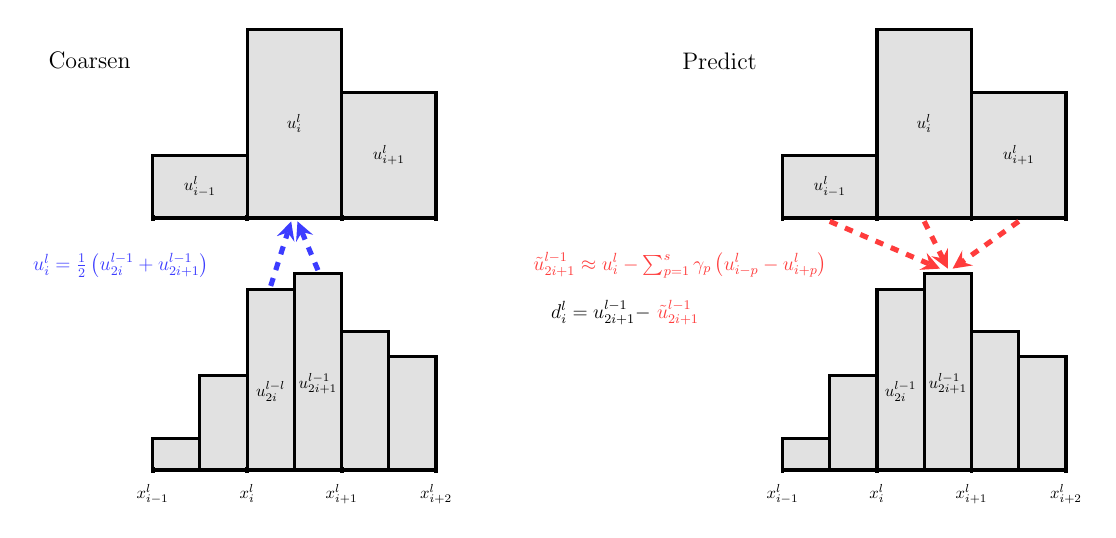
\begin{tikzpicture}[thick,scale=0.4, every node/.style={scale=0.6}]
    
        % variables
        \def\x{-17.0}
        \def\y{0.0}
        \def\yl{-8.0}
        
        % draw coarse level rectangles
        \draw [fill=mygray,line width=0.4mm] (\x,0) rectangle (\x+3,2);
        \draw [fill=mygray,line width=0.4mm] (\x+3,0) rectangle (\x+6,6);
        \draw [fill=mygray,line width=0.4mm] (\x+6,0) rectangle (\x+9,4);
        
        % arrows
        \draw[myblue,dashed,->,line width=0.65mm,>=stealth] (\x+5.25,\y-1.65) -- (\x+4.6,\y-0.1);
        \draw[myblue,dashed,->,line width=0.65mm,>=stealth] (\x+3.75,\y-2.15) -- (\x+4.40,\y-0.1);
        
        % coarse level symbols
        \node at (\x+1.5,1) { $u^{l}_{i-1}$};
        \node at (\x+4.5,3) { $u^{l}_{i}$};
        \node at (\x+7.5,2) { $u^{l}_{i+1}$};

        % fine level rectangles
        \draw [fill=mygray,line width=0.4mm] (\x,\yl) rectangle (\x+1.5,\yl+1);
        \draw [fill=mygray,line width=0.4mm] (\x+1.5,\yl) rectangle (\x+3,\yl+3);
        \draw [fill=mygray,line width=0.4mm] (\x+3,\yl) rectangle (\x+4.5,\yl+5.75);
        \draw [fill=mygray,line width=0.4mm] (\x+4.5,\yl) rectangle (\x+6,\yl+6.25);
        \draw [fill=mygray,line width=0.4mm] (\x+6,\yl) rectangle (\x+7.5,\yl+4.4);
        \draw [fill=mygray,line width=0.4mm] (\x+7.5,\yl) rectangle (\x+9,\yl+3.6);
        
        % coarse level axis
        \draw[line width=0.5mm] (\x,0) -- (\x+9,0);
        \draw[line width=0.5mm] (\x,.1) -- (\x,-0.1);
        \draw[line width=0.5mm] (\x+3,0.1) -- (\x+3,-0.1);
        \draw[line width=0.5mm] (\x+6,0.1) -- (\x+6,-0.1);
        \draw[line width=0.5mm] (\x+9,0.1) -- (\x+9,-0.1);
        
        % fine level symbols
        \node at (\x+3.75,\yl+2.5) { $u^{l-l}_{2i}$};
        \node at (\x+5.25,\yl+2.75) { $u^{l-1}_{2i+1}$};
        
        % fine level axis
        \draw[line width=0.5mm] (\x,\yl) -- (\x+9,\yl);
        \draw[line width=0.5mm] (\x,\yl+.1) -- (\x,\yl-0.1);
        \draw[line width=0.5mm] (\x+3,\yl+.1) -- (\x+3,\yl-0.1);
        \draw[line width=0.5mm] (\x+6,\yl+.1) -- (\x+6,\yl-0.1);
        \draw[line width=0.5mm] (\x+9,\yl+.1) -- (\x+9,\yl-0.1);

        % tick text
        \node[below] at (\x,\yl-0.25) {$x^{l}_{i-1}$};
        \node[below] at (\x+3,\yl-0.25) { $x^{l}_{i}$};
        %\node[below] at (\x+4.5,\yl-0.25) { $x^{l}_{k+1/2}$};
        \node[below] at (\x+6,\yl-0.25) { $x^{l}_{i+1}$};
        \node[below] at (\x+9,\yl-0.25) { $x^{l}_{i+2}$};
        
        %----
        
        % variables
        \def\x{3.0}
        \def\y{0.0}
        \def\yl{-8.0}
        
        % draw coarse level rectangles
        \draw [fill=mygray,line width=0.4mm] (\x,0) rectangle (\x+3,2);
        \draw [fill=mygray,line width=0.4mm] (\x+3,0) rectangle (\x+6,6);
        \draw [fill=mygray,line width=0.4mm] (\x+6,0) rectangle (\x+9,4);
        
        % coarse level symbols
        \node at (\x+1.5,1) {$u^{l}_{i-1}$};
        \node at (\x+4.5,3) { $u^{l}_{i}$};
        \node at (\x+7.5,2) { $u^{l}_{i+1}$};
        
        % coarse level axis
        \draw[line width=0.5mm] (\x,0) -- (\x+9,0);
        \draw[line width=0.5mm] (\x,.1) -- (\x,-0.1);
        \draw[line width=0.5mm] (\x+3,0.1) -- (\x+3,-0.1);
        \draw[line width=0.5mm] (\x+6,0.1) -- (\x+6,-0.1);
        \draw[line width=0.5mm] (\x+9,0.1) -- (\x+9,-0.1);

        % fine level rectangles
        \draw [fill=mygray,line width=0.4mm] (\x,\yl) rectangle (\x+1.5,\yl+1);
        \draw [fill=mygray,line width=0.4mm] (\x+1.5,\yl) rectangle (\x+3,\yl+3);
        \draw [fill=mygray,line width=0.4mm] (\x+3,\yl) rectangle (\x+4.5,\yl+5.75);
        \draw [fill=mygray,line width=0.4mm] (\x+4.5,\yl) rectangle (\x+6,\yl+6.25);
        \draw [fill=mygray,line width=0.4mm] (\x+6,\yl) rectangle (\x+7.5,\yl+4.4);
        \draw [fill=mygray,line width=0.4mm] (\x+7.5,\yl) rectangle (\x+9,\yl+3.6);
        
        % fine level symbols
        \node at (\x+3.75,\yl+2.5) { $u^{l-1}_{2i}$};
        \node at (\x+5.25,\yl+2.75) { $u^{l-1}_{2i+1}$};
        
        % fine level axis
        \draw[line width=0.5mm] (\x,\yl) -- (\x+9,\yl);
        \draw[line width=0.5mm] (\x,\yl+.1) -- (\x,\yl-0.1);
        \draw[line width=0.5mm] (\x+3,\yl+.1) -- (\x+3,\yl-0.1);
        \draw[line width=0.5mm] (\x+6,\yl+.1) -- (\x+6,\yl-0.1);
        \draw[line width=0.5mm] (\x+9,\yl+.1) -- (\x+9,\yl-0.1);

        % arrows
        \draw[myred,dashed,->,line width=0.65mm,>=stealth] (\x+1.5,\y-0.1) -- (\x+5,\y-1.6);
        \draw[myred,dashed,->,line width=0.65mm,>=stealth] (\x+4.5,\y-0.1) -- (\x+5.25,\y-1.6);
        \draw[myred,dashed,->,line width=0.65mm,>=stealth] (\x+7.5,\y-0.1) -- (\x+5.4,\y-1.6);

        % tick text
        \node[below] at (\x,\yl-0.25) { $x^{l}_{i-1}$};
        \node[below] at (\x+3,\yl-0.25) { $x^{l}_{i}$};
        %\node[below] at (\x+4.5,\yl-0.25) { $x^{l}_{i+1/2}$};
        \node[below] at (\x+6,\yl-0.25) { $x^{l}_{i+1}$};
        \node[below] at (\x+9,\yl-0.25) { $x^{l}_{i+2}$};
        
        % text
        \node at (\x-2.0,\y+5.0) {\Large Predict};
        \node at (\x-22,\y+5.0) {\Large Coarsen};
        
        % math
        \node at (\x-3.25,\yl+6.5) {\large \color{myred} $\tilde{u}_{2i+1}^{l-1} \approx u_{i}^{l} - \sum_{p=1}^{s} \gamma_{p} \left( u^{l}_{i-p} - u^{l}_{i+p} \right)$ };
        
        \node at (\x-5,\yl+5.0) {\large $d_{i}^{l} = u_{2i+1}^{l-1} - $\color{myred}$ \text{ } \tilde{u}_{2i+1}^{l-1}$};
        
        \node at (\x-21,\yl+6.5) {\large \color{myblue} $u_{i}^{l} = \frac{1}{2} \left( u_{2i}^{l-1} + u_{2i+1}^{l-1} \right)$};

    \end{tikzpicture}

    \caption{Left: quadratic prediction from coarse-scale $j$
        to fine-scale $j+1$, given cell-averages $\mathbf{c}^{j}$.
        Right: Fine-scale cell averages are coarsened.}
\end{figure}

\section{Numerical Tests}
\begin{center}\vspace{1cm}
\begin{tabular}{|l|l|l|l|l|l|l|l|l|}
\hline
           & \multicolumn{4}{l|}{$\epsilon = 0.0$}              & \multicolumn{4}{l|}{$\epsilon = 10^{-12}$}         \\ \hline
grid cells & $L_{1}$ error & order & $L_{\infty}$ error & order & $L_{1}$ error & order & $L_{\infty}$ error & order \\ \hline
16         &               &       &                    &       &               &       &                    &       \\ \hline
32         &               &       &                    &       &               &       &                    &       \\ \hline
64         &               &       &                    &       &               &       &                    &       \\ \hline
128        &               &       &                    &       &               &       &                    &       \\ \hline
256        &               &       &                    &       &               &       &                    &       \\ \hline
           & \multicolumn{4}{l|}{$\epsilon = 10^{-6}$}          & \multicolumn{4}{l|}{$\epsilon = 10^{-4}$}          \\ \hline
grid cells & $L_{1}$ error & order & $L_{\infty}$ error & order & $L_{1}$ error & order & $L_{\infty}$ error & order \\ \hline
16         &               &       &                    &       &               &       &                    &       \\ \hline
32         &               &       &                    &       &               &       &                    &       \\ \hline
64         &               &       &                    &       &               &       &                    &       \\ \hline
128        &               &       &                    &       &               &       &                    &       \\ \hline
256        &               &       &                    &       &               &       &                    &       \\ \hline
\end{tabular}
\end{center}\vspace{1cm}

\subsection{Example}
Using the inviscid flow assumption, the dynamics of compressible fluids are
modeled using the reactive Euler equations \hl{add domain notation}
\begin{equation}
   u_{t} + f(u)_{x}
   + g(u)_{y} = s(u),
    \label{goveq}
\end{equation}
where $u = \left( \rho, \rho u, \rho v, \rho w, E \right)^{T}$ is
the state vector, the flux vectors are given by
\begin{equation}
    f = 
\begin{pmatrix}
\rho u \\ \rho u^2 + p \\ \rho u v \\ \rho u w \\ u( E + p )
\end{pmatrix}, \text{ } \text{ } \text{ }
    g = 
\begin{pmatrix}
\rho v \\ \rho u v \\ \rho v^2 + p \\ \rho v w \\ v( E + p )
\end{pmatrix}, \text{ } \text{ } \text{ }
    h = 
\begin{pmatrix}
\rho w \\ \rho u w \\ \rho v w \\ \rho w^2 + p \\ w( E + p )
\end{pmatrix},
\end{equation}
and $s(u)$ represents sources. The total energy per
unit volume is given by
\begin{equation*}
    E = \rho \left( \frac{1}{2} \mathbf{V}^{2} + e \right),
\end{equation*}
where $e$ is the internal energy and the kinetic energy contribution is
\begin{equation*}
    \frac{1}{2} \mathbf{V}^{2} = \frac{1}{2} \mathbf{V}
    \cdot \mathbf{V} = \frac{1}{2} \left( u^2 + v^2 + w^2 \right).
\end{equation*}
The system of nonlinear equations is closed by an
equation of state which is in general not derived from that of an ideal gas.
\begin{figure}[H]
    \center
    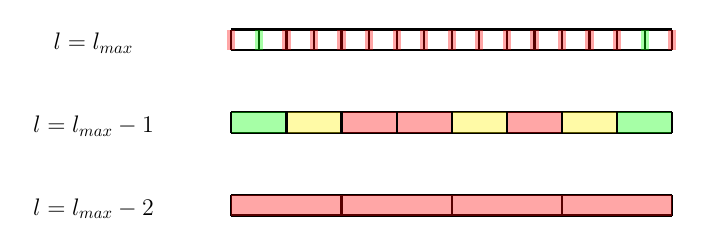
\begin{tikzpicture}[thick,scale=0.35, every node/.style={scale=0.6}]
    
        % variables
        \def\xl{-8.0}
        \def\xr{8.0}
        \def\y{0.0}
        \def\yy{-3.0}
        \def\yyy{-6.0}
        \def\ts{0.75}
        \def\op{0.35}
        \def\fx{0.15}
        
        % draw grids
        \draw (\xl,\y) --(\xr,\y);
        \draw (\xl,\y+\ts) --(\xr,\y+\ts);
        \draw (\xl,\yy) --(\xr,\yy);
        \draw (\xl,\yy+\ts) --(\xr,\yy+\ts);
        \draw (\xl,\yyy) --(\xr,\yyy);
        \draw (\xl,\yyy+\ts) --(\xr,\yyy+\ts);
        
        % draw cells for max level
        \draw (\xl,\y) --(\xl,\y+\ts);
        \draw (\xl+1.0,\y) --(\xl+1.0,\y+\ts);
        \draw (\xl+2.0,\y) --(\xl+2.0,\y+\ts);
        \draw (\xl+3.0,\y) --(\xl+3.0,\y+\ts);
        \draw (\xl+4.0,\y) --(\xl+4.0,\y+\ts);
        \draw (\xl+5.0,\y) --(\xl+5.0,\y+\ts);
        \draw (\xl+6.0,\y) --(\xl+6.0,\y+\ts);
        \draw (\xl+7.0,\y) --(\xl+7.0,\y+\ts);
        \draw (\xl+8.0,\y) --(\xl+8.0,\y+\ts);
        \draw (\xl+9.0,\y) --(\xl+9.0,\y+\ts);
        \draw (\xl+10.0,\y) --(\xl+10.0,\y+\ts);
        \draw (\xl+11.0,\y) --(\xl+11.0,\y+\ts);
        \draw (\xl+12.0,\y) --(\xl+12.0,\y+\ts);
        \draw (\xl+13.0,\y) --(\xl+13.0,\y+\ts);
        \draw (\xl+14.0,\y) --(\xl+14.0,\y+\ts);
        \draw (\xl+15.0,\y) --(\xl+15.0,\y+\ts);
        \draw (\xl+16.0,\y) --(\xl+16.0,\y+\ts);
        
        % color in cells at level L-1
        \fill [green, opacity=\op] (\xl,\yy) rectangle (\xl+2.0,\yy+\ts);
        \fill [yellow, opacity=\op] (\xl+2.0,\yy) rectangle (\xl+4.0,\yy+\ts);
        \fill [red, opacity=\op] (\xl+4.0,\yy) rectangle (\xl+6.0,\yy+\ts);
        \fill [red, opacity=\op] (\xl+6.0,\yy) rectangle (\xl+8.0,\yy+\ts);
        \fill [yellow, opacity=\op] (\xl+8.0,\yy) rectangle (\xl+10.0,\yy+\ts);
        \fill [red, opacity=\op] (\xl+10.0,\yy) rectangle (\xl+12.0,\yy+\ts);
        \fill [yellow, opacity=\op] (\xl+12.0,\yy) rectangle (\xl+14.0,\yy+\ts);
        \fill [green, opacity=\op] (\xl+14.0,\yy) rectangle (\xl+16.0,\yy+\ts);
        
        % lower level cells
        \draw (\xl,\yy) --(\xl,\yy+\ts);
        \draw (\xl+2.0,\yy) --(\xl+2.0,\yy+\ts);
        \draw (\xl+4.0,\yy) --(\xl+4.0,\yy+\ts);
        \draw (\xl+6.0,\yy) --(\xl+6.0,\yy+\ts);
        \draw (\xl+8.0,\yy) --(\xl+8.0,\yy+\ts);
        \draw (\xl+10.0,\yy) --(\xl+10.0,\yy+\ts);
        \draw (\xl+12.0,\yy) --(\xl+12.0,\yy+\ts);
        \draw (\xl+14.0,\yy) --(\xl+14.0,\yy+\ts);
        \draw (\xl+16.0,\yy) --(\xl+16.0,\yy+\ts);
        
        % even lower level cells
        \draw (\xl,\yyy) --(\xl,\yyy+\ts);
        \draw (\xl+4.0,\yyy) --(\xl+4.0,\yyy+\ts);
        \draw (\xl+8.0,\yyy) --(\xl+8.0,\yyy+\ts);
        \draw (\xl+12.0,\yyy) --(\xl+12.0,\yyy+\ts);
        \draw (\xl+16.0,\yyy) --(\xl+16.0,\yyy+\ts);
        
        % color in cells at level L-2
        \fill [red, opacity=\op] (\xl,\yyy) rectangle (\xl+4.0,\yyy+\ts);
        \fill [red, opacity=\op] (\xl+4.0,\yyy) rectangle (\xl+8.0,\yyy+\ts);
        \fill [red, opacity=\op] (\xl+8.0,\yyy) rectangle (\xl+12.0,\yyy+\ts);
        \fill [red, opacity=\op] (\xl+12.0,\yyy) rectangle (\xl+16.0,\yyy+\ts);
        
        % draw colored fluxes
        \fill [red, opacity=\op] (\xl+0.0-\fx,\y) rectangle (\xl+0.0+\fx,\y+\ts);
        \fill [green, opacity=\op] (\xl+1.0-\fx,\y) rectangle (\xl+1.0+\fx,\y+\ts);
        \fill [red, opacity=\op] (\xl+2.0-\fx,\y) rectangle (\xl+2.0+\fx,\y+\ts);
        \fill [red, opacity=\op] (\xl+3.0-\fx,\y) rectangle (\xl+3.0+\fx,\y+\ts);
        \fill [red, opacity=\op] (\xl+4.0-\fx,\y) rectangle (\xl+4.0+\fx,\y+\ts);
        \fill [red, opacity=\op] (\xl+5.0-\fx,\y) rectangle (\xl+5.0+\fx,\y+\ts);
        \fill [red, opacity=\op] (\xl+6.0-\fx,\y) rectangle (\xl+6.0+\fx,\y+\ts);
        \fill [red, opacity=\op] (\xl+7.0-\fx,\y) rectangle (\xl+7.0+\fx,\y+\ts);
        \fill [red, opacity=\op] (\xl+8.0-\fx,\y) rectangle (\xl+8.0+\fx,\y+\ts);
        \fill [red, opacity=\op] (\xl+9.0-\fx,\y) rectangle (\xl+9.0+\fx,\y+\ts);
        \fill [red, opacity=\op] (\xl+10.0-\fx,\y) rectangle (\xl+10.0+\fx,\y+\ts);
        \fill [red, opacity=\op] (\xl+11.0-\fx,\y) rectangle (\xl+11.0+\fx,\y+\ts);
        \fill [red, opacity=\op] (\xl+12.0-\fx,\y) rectangle (\xl+12.0+\fx,\y+\ts);
        \fill [red, opacity=\op] (\xl+13.0-\fx,\y) rectangle (\xl+13.0+\fx,\y+\ts);
        \fill [red, opacity=\op] (\xl+14.0-\fx,\y) rectangle (\xl+14.0+\fx,\y+\ts);
        \fill [green, opacity=\op] (\xl+15.0-\fx,\y) rectangle (\xl+15.0+\fx,\y+\ts);
        \fill [red, opacity=\op] (\xl+16.0-\fx,\y) rectangle (\xl+16.0+\fx,\y+\ts);
        
        % nodes
        \node at (\xl-5.0,\y+0.25) {\Large $l=l_{max}$};
        \node at (\xl-5.0,\yy+0.25) {\Large $l=l_{max}-1$};
        \node at (\xl-5.0,\yyy+0.25) {\Large $l=l_{max}-2$};

    \end{tikzpicture}
    \caption{An illustrative case of the multiresolution decomposition applied to a block of data 16 cells wide, showing two coarser grid levels, with green and red cells indicating insignificant and significant detail coefficients, respectively. Yellow cells represent the buffer region surrounding a cell with a large detail coefficient.}
\end{figure}

\begin{figure}[H]
    \centering
    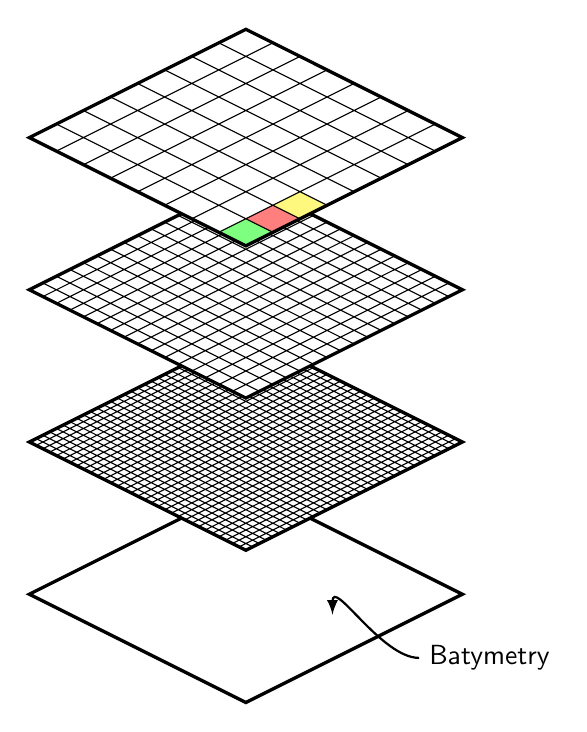
\begin{tikzpicture}[scale=.55,every node/.style={minimum size=1cm},on grid]
            	
    \begin{scope}[
        yshift=-200,every node/.append style={
        yslant=0.5,xslant=-1},yslant=0.5,xslant=-1 ]
        %marking border
        \draw[black,very thick] (0,0) rectangle (5,5);
    \end{scope} %end of drawing grids
    
    \begin{scope}[
    	yshift=-100,every node/.append style={
    	    yslant=0.5,xslant=-1},yslant=0.5,xslant=-1 ]
        \fill[white,fill opacity=1.0] (0,0) rectangle (5,5);
        \draw[black,very thick] (0,0) rectangle (5,5);
        \draw[step=1.5625mm, black] (0,0) grid (5,5);
    \end{scope}
    
    \begin{scope}[
    	yshift=0,every node/.append style={
    	    yslant=0.5,xslant=-1},yslant=0.5,xslant=-1 ]
        \fill[white,fill opacity=1.0] (0,0) rectangle (5,5);
        \draw[black,very thick] (0,0) rectangle (5,5);
        \draw[step=3.125mm, black] (0,0) grid (5,5);
    \end{scope}
    
    \begin{scope}[
    	yshift=100,every node/.append style={
    	    yslant=0.5,xslant=-1},yslant=0.5,xslant=-1 ]
        \fill[white,fill opacity=1.0] (0,0) rectangle (5,5);
        \fill[green,fill opacity=0.5] (0,0) rectangle (0.625,0.625);
        \fill[red,fill opacity=0.5] (0.625,0) rectangle(1.25,0.625);
        \fill[yellow,fill opacity=0.5] (1.25,0) rectangle(1.875,0.625);
        \draw[black,very thick] (0,0) rectangle (5,5);
        \draw[step=6.25mm, black] (0,0) grid (5,5);
    \end{scope}

    \draw[-latex,thick](4,-6)node[right]{$\mathsf{Batymetry}$}
        to[out=180,in=90] (2,-5);	
	
    \end{tikzpicture}
    \caption{Wavelet decomposition of a $32\times 32$ block of cells with three grid levels. Coloring indicates cells with a significant detail
                coefficient (red), cells in the buffer region (yellow), and cells with a small detail coefficient that are not in the buffer region (green).}
\end{figure}

\section{Acknowledgements}

\appendix

\section{Literature Review}

\section{Derivation of Prediction Operator in One-Dimension}
We are interested in obtaining the difference between approximation spaces at varying levels of resolution. We 
are given cell-averaged values as input data to our wavelet transform. This data is fed to the scheme at some arbitrary maximum
resolution level $J$, and the wavelet transform produces details coefficients at each lower level until the coarsest level,
$j=0$, is reached. The coefficients in this case are interchangeable with the cell-averages and are denoted by $c^{j}_{k}$,
where the level of resolution is denoted by $j$, and the spatial index is denoted by $k$. We consider an interpolating
polynomial $p(x)$ such that 
\begin{align}
    c^{j}_{k-1} &= \int_{x^{j}_{k-1}}^{x^{j}_{k}} p(x) dx \\
    c^{j}_{k} &= \int_{x^{j}_{k}}^{x^{j}_{k+1}} p(x) dx \\
    c^{j}_{k+1} &= \int_{x^{j}_{k+1}}^{x^{j}_{k+2}} p(x) dx.
\end{align}
The polynomial $p(x)$ should then predict the finer cell-averages of cell $c^{j}_{k}$ as
\begin{align}
    \hat{c}^{j+1}_{2k} &= 2 \int_{x^{j}_{k}}^{x^{j}_{k+1/2}} p(x) dx \\
    \hat{c}^{j+1}_{2k+1} &= 2 \int_{x^{j}_{k+1/2}}^{x^{j}_{k+1}} p(x) dx
\end{align}
At present, it may not be clear how to implement such a scheme on a computer. However this interpolation procedure
can be cast in a more suitable form by introducing another polynomial, the integral of $p(x)$:
\begin{equation}
	P(x) = \int_{0}^{x} p(y) dy.
\end{equation}
Now the problem is to interpolate the following data
\begin{align}
    0 &= P(x^{j}_{k-1}) \\
    c^{j}_{k-1} &= P(x^{j}_{k}) \\
    c^{j}_{k-1} + c^{j}_{k} &= P(x^{j}_{k+1}) \\
    c^{j}_{k-1} + c^{j}_{k} + c^{j}_{k+1} &= P(x^{j}_{k+2}).
\end{align}
This can easily be done using Lagrange polynomials. Then the predictions are given in terms of $P(x)$ by
\begin{align}
	\hat{c}^{j+1}_{2k} &= 2 \left( P(x^{j}_{k+1/2}) - P(x^{j}_{k}) \right) \\
	\hat{c}^{j+1}_{2k+1} &= 2 \left( P(x^{j}_{k+1}) - P(x^{j}_{k+1/2}) \right).
\end{align}
This interpolating polynomial is cast in the Lagrange form,
\begin{equation}
P(x) = \sum_{i=0}^{n} y_{i} l_{i}(x),
\end{equation}
where $y_{i}$ are the functional data, and $l_{i}(x)$ are the Lagrange polynomials. For $n=3$ these
are given by
\begin{align}
    l_{0}(x) &= \frac{x-x_1}{x_0-x_1} \frac{x-x_2}{x_0-x_2} \frac{x-x_3}{x_0-x_3} \\
    l_{1}(x) &= \frac{x-x_0}{x_1-x_0} \frac{x-x_2}{x_1-x_2} \frac{x-x_3}{x_1-x_3} \\
    l_{2}(x) &= \frac{x-x_0}{x_2-x_0} \frac{x-x_1}{x_2-x_1} \frac{x-x_3}{x_2-x_3} \\
    l_{3}(x) &= \frac{x-x_0}{x_3-x_0} \frac{x-x_1}{x_3-x_1} \frac{x-x_2}{x_3-x_2},
\end{align}
and the final interpolating polynomial is
\begin{equation}
	P(x) = (0) l_{0}(x) + ( c^{j}_{k-1} ) l_{1}(x) + ( c^{j}_{k-1} + c^{j}_{k} ) l_{2}(x)
		+ ( c^{j}_{k-1} + c^{j}_{k} + c^{j}_{k+1} ) l_{3}(x).
\end{equation}
Several evaluations are necessary in order to obtain the predictions. Using intervals of equal length, these values are
\begin{align}
	P(x^{j}_{k}) &= c^{j}_{k-1} \\
	P(x^{j}_{k+1/2}) &= \frac{17}{16} c^{j}_{k-1} + \frac{1}{2} c^{j}_{k} - \frac{1}{16} c^{j}_{k+1} \\
	P(x^{j}_{k+1}) &= c^{j}_{k-1} + c^{j}_{k}.
\end{align}
Then the predictions of the cell-averages at the higher level of resolution are finally given by
\begin{align}
	\hat{c}^{j+1}_{2k} & = c^{j}_{k} + \frac{1}{8} \left( c^{j}_{k-1} - c^{j}_{k+1} \right) \\
	\hat{c}^{j+1}_{2k+1} & = c^{j}_{k} - \frac{1}{8} \left( c^{j}_{k-1} - c^{j}_{k+1} \right).
\end{align}
This procedure could easily be extended to non-uniformly
spaced intervals, giving different weights. Note that only the
odd indices are counted because in the multiresolution scheme the
data is initially split into even
and odd signals. All data at level $j$ are just considered to
be a copy of the even-index data at level $j+1$, whereas
the odd-indexed data at level $j+1$ is what is predicted
by even-indexed data at level $j+1$. Also important are the
interpolants at the ends of the domain. Given below are the
left and right predictions, respectively:
\begin{align}
	\hat{c}^{j+1}_{2k+1} & = \frac{5}{8} c^{j}_{k}
	+ \frac{1}{2} c^{j}_{k+1} - \frac{1}{8} c^{j}_{k+2} \\
	\hat{c}^{j+1}_{2k+1} & = \frac{1}{8} c^{j}_{k-2}
	- \frac{1}{2} c^{j}_{k-1} + \frac{11}{8} c^{j}_{k}.
\end{align}

\bibliographystyle{unsrt}  
\bibliography{references}

\end{document}
